\frame{
    \frametitle{Dealing with the donut!}
    \begin{columns}
        \begin{column}{0.6\textwidth}
            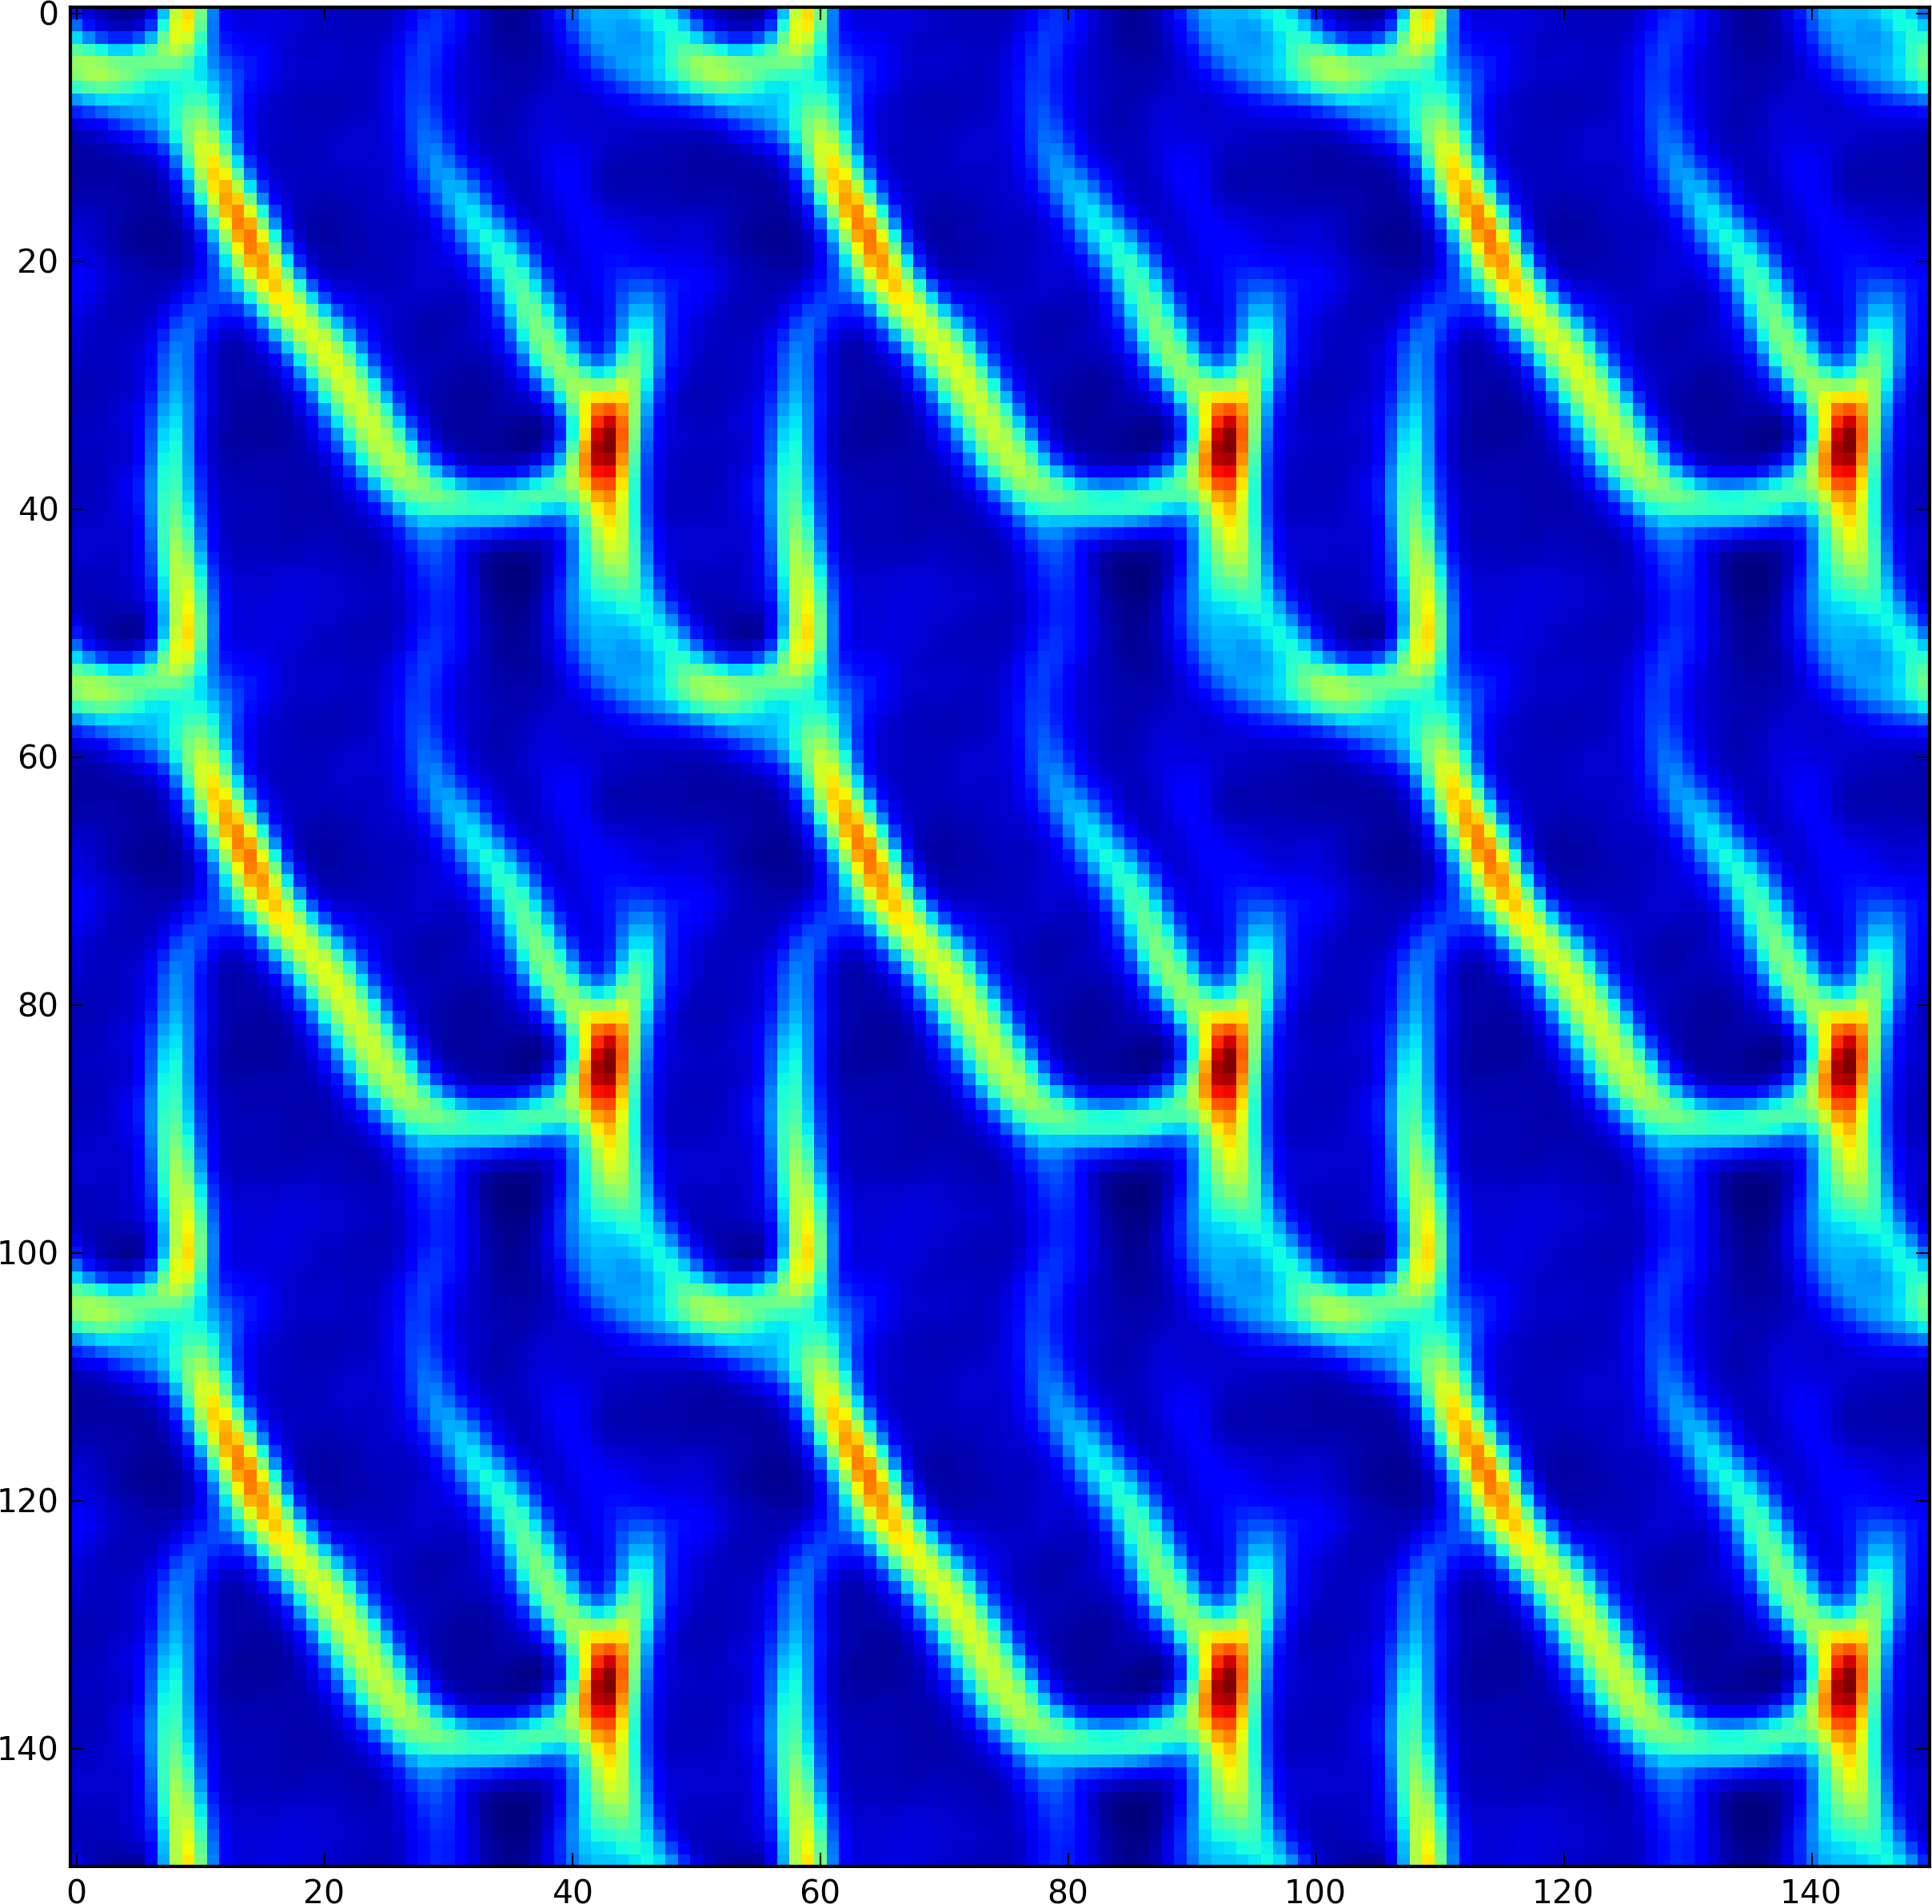
\includegraphics[width=\textwidth]{figures/umat_expand.png}
        \end{column}
        \begin{column}{0.4\textwidth}
            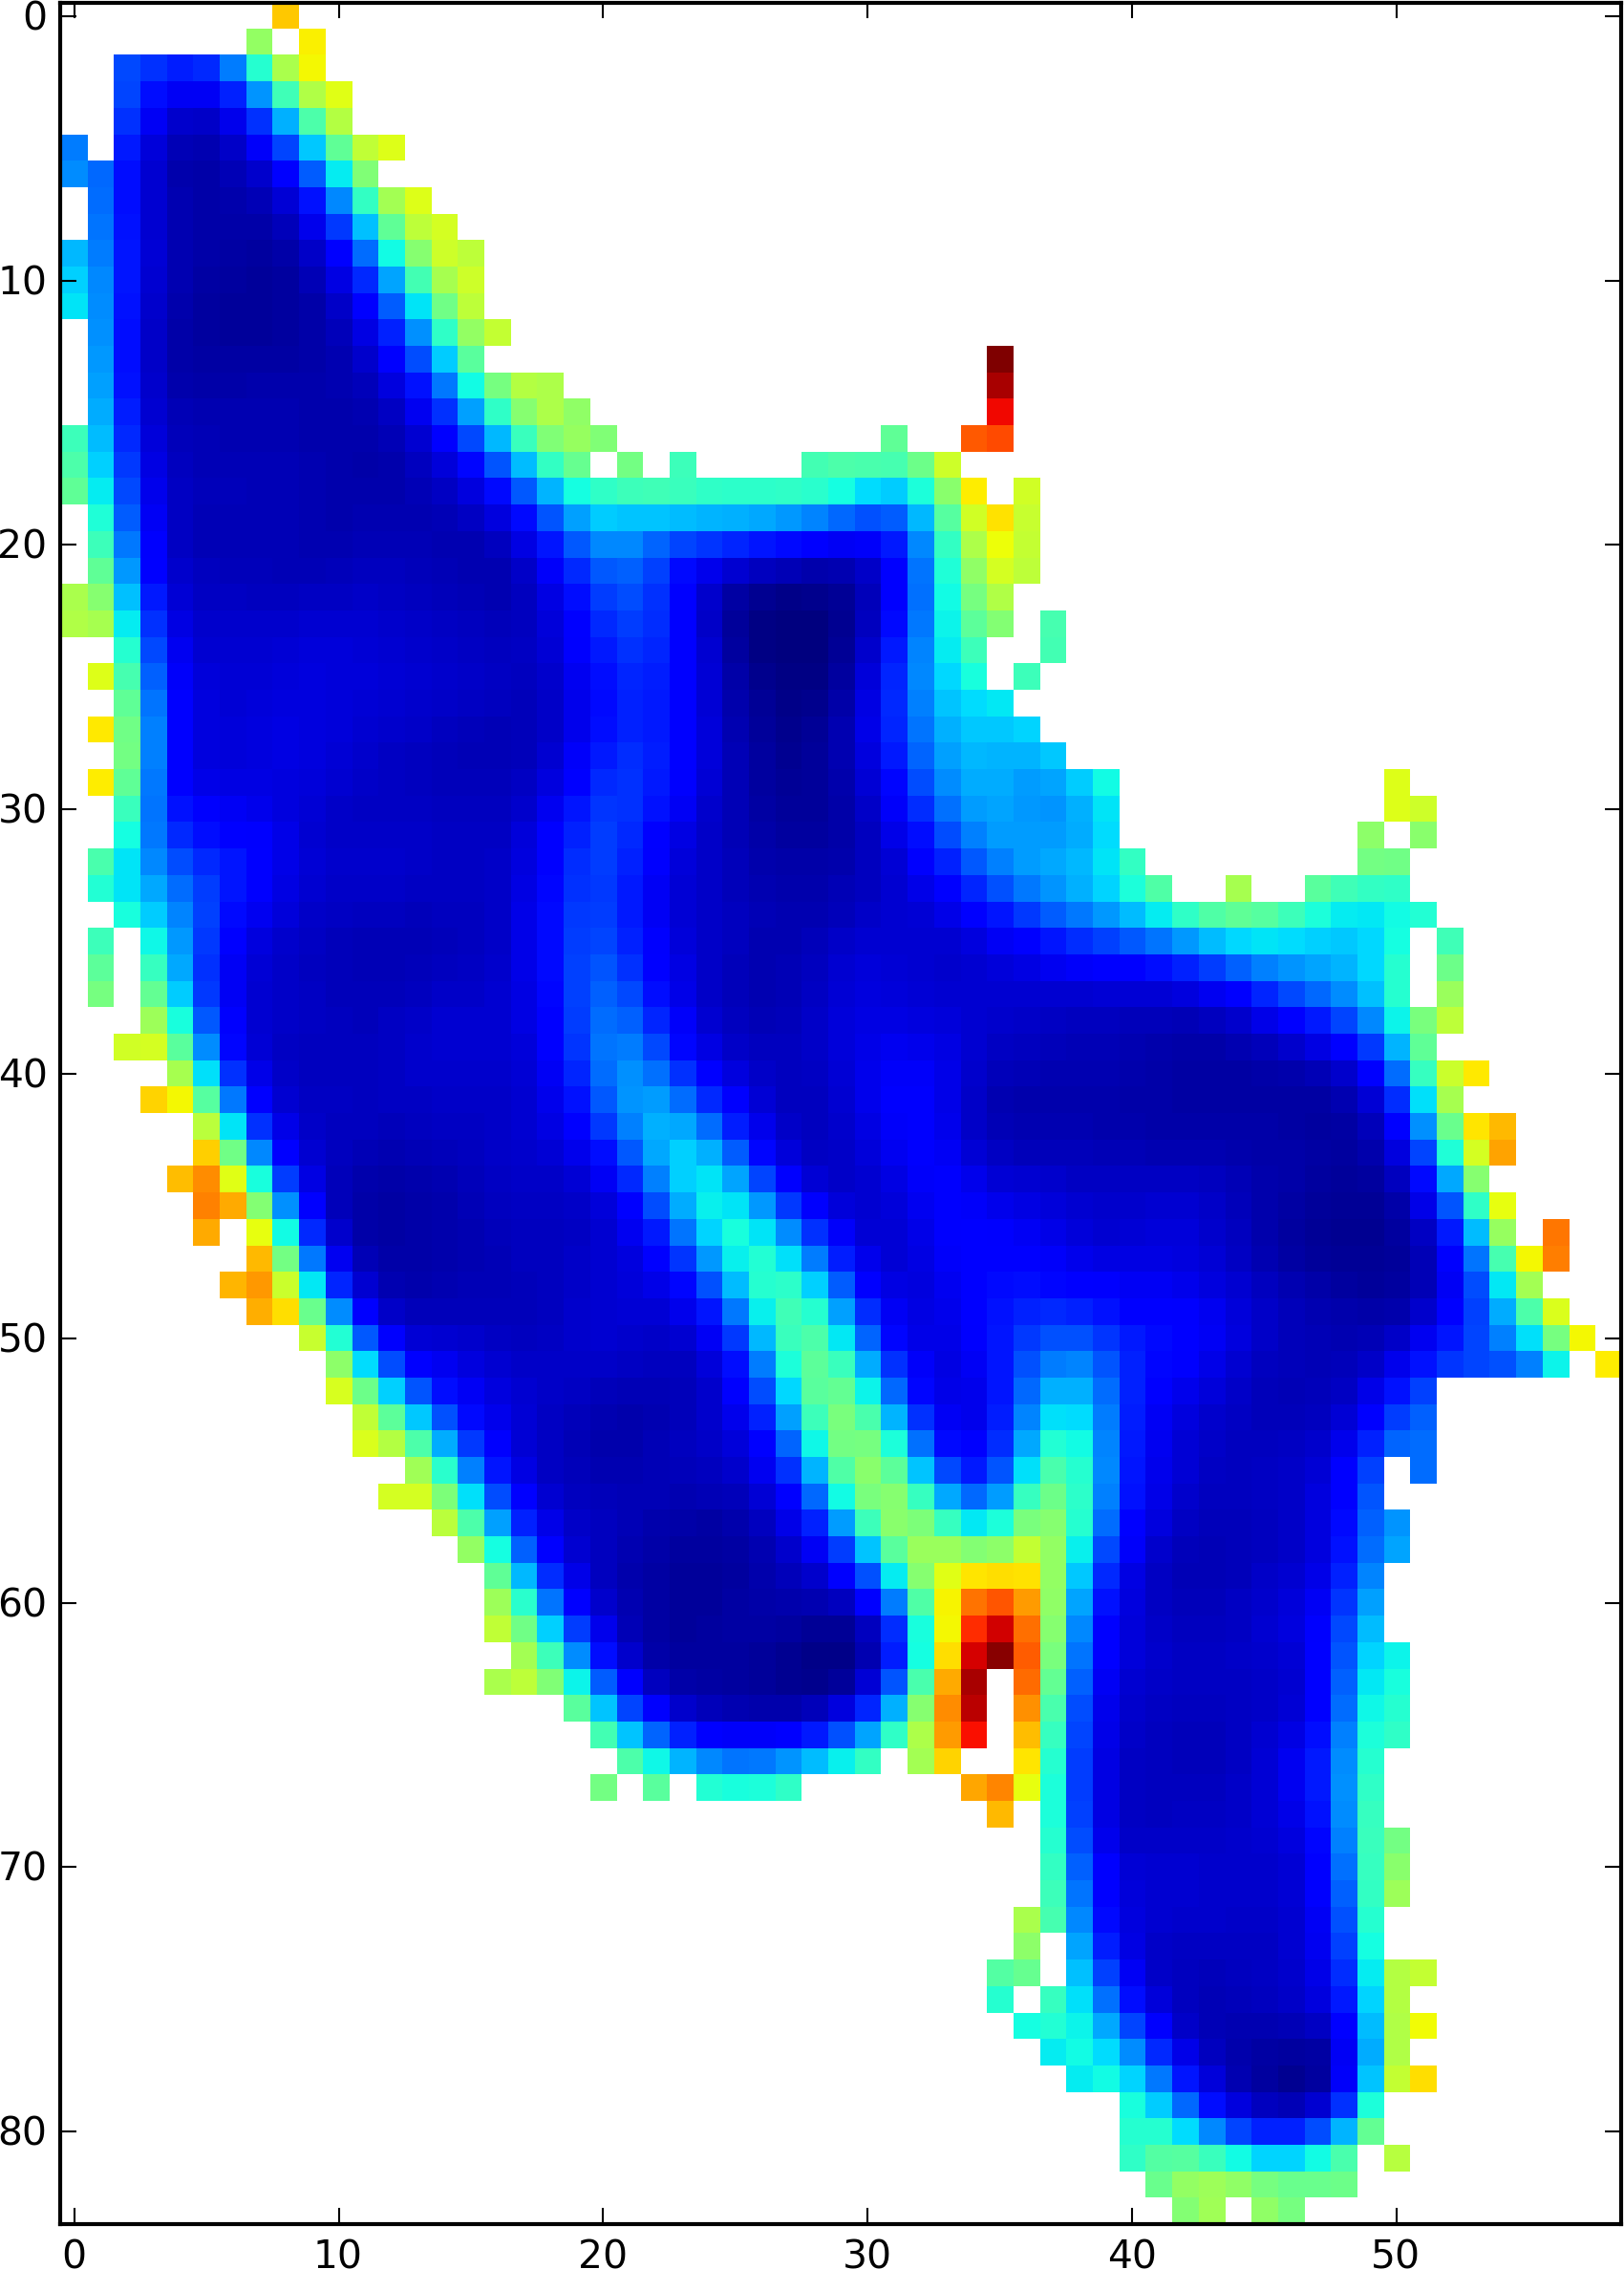
\includegraphics[width=\textwidth]{figures/umat_cont.png}
        \end{column}
    \end{columns}
    The algorithm -- called ``flooding algorithm'' -- starts from the global minimum of the U-matrix (many thanks to Mathias Ferber for this idea).
    It floods the map according to the relief of the U-matrix.
    This algorithm is inspired from the watershed algorithm.
}
